The Australian Ovarian Cancer Study (AOCS)\cite{Patch_2015} performed whole genome sequencing on 92 high grade serous Ovarian cancer tumors, including 15 donors with matched primary and acquired resistance samples. Their analysis found that the recurrence samples harbored more somatic mutations than the primary samples and were enriched for mutations in a $C(C \gt T)C$ context, suggestive of a possible impact of chemotherapy. We extend this analysis by quantifying the number of potential neoantigen-generating mutations in the primary and recurrence samples and testing whether mutational signature deconvolution attributes the unique-to-recurrence mutations to the \texit{C. Elegans} cisplatin signature. We include three additional donors from TCGA and one donor from our institution in our analysis (\ref{tab:cohort}).

Ideally we would have some non-chemo treated surigical patients to serve as control. As platinum chemo is standard of care, we have to use signatures to figure out if it's likely due to chemo.

As surgery is not usually performed for relapsed disease, the AOCS relapsed samples consist predominantly of drained ascites samples. We analyze ascites separately from solid tumors to avoid confounding.



\section*{Results}

\subsection*{Change in mutations and neoantigens at recurrence}
To investigate changes in mutational burden and neoantigens associated with recurrence after treatment, we performed paired and unpaired analyses as well as a Bayesian regression integrating both paired and unpaired samples (Figure \ref{fig:bayesian}). The Bayesian analysis controls for whether the tissue was solid tumor or ascites, sample purity, the number of samples from the same donor, and also probes an interaction between tissue type and recurrence. In this model, chemotherapy treated samples had 47\% (-2-125) more detectable mutations than primary samples.

Across our cohort of 115 samples from 93 donors, we identified 20,672 potential neoantigens, defined as mutated peptides predicted to bind autologous MHC class I with affinity $\leq 500$nm (Table \ref{tab:cohort}). All but 29 (0.14\%) neoantigens were private to a single donor. As expected, the number of neoantigens tracked the increase in mutational burden at relapse. In the Bayesian analysis, treated samples had 49\% (-19-182) more neoantigens, and, for ascites samples, 104\% (2-300) more expressed neoantigens. For solid tumor samples, the total number of neoantigens increased 



\subsection*{Mutation signatures}
To explore possible etiologies for the increased mutational burden at recurrence, we deconvolved the mutations present in each sample into known signatures. We used the 30 signatures curated by COSMIC (http://cancer.sanger.ac.uk/cosmic/signatures), plus four additional signatures we manually extracted from a study of cisplatin-exposed \textit{C. Elegans} [Meier et al], and chicken exposed to several mutagenic chemotherapies. Consistent with results originally reported by Patch et al on this cohort, the mutations were attributable mostly to Signatures 1 and 3, which are associated with Age and BRCA disruption, respectively. These two signatures together accounted for 82\% (75-88) of the mutations in primary samples and 70\% (64-76) of the mutations unique to the relapses. The remaining mutations in the relapses were attributed to different signatures in various samples. Signature 4, associated with smoking, was the only additional signature consistently given nonzero weight in the relapse samples. In the 9 relapse samples in which it was assigned nonzero weight, Signature 4 accounted for 10\% (8-13) of the unique-to-relapse mutations. Two primary samples also showed evidence for Signature 4. Smoking history of these patients was not known.



\begin{table}
\begin{tabular}{llllll}
\toprule
{} & donors & samples (RNA) &            Mutations &    Neoantigens & Expressed neoantigens \\
\midrule
ascites untreated      &      4 &         4 (4) &   10336 (9600-11000) &  205 (140-270) &           82 (50-110) \\
ascites post-treatment &     22 &       25 (20) &  13757 (12000-15000) &  303 (260-350) &         149 (120-180) \\
solid untreated        &     75 &       75 (69) &     7902 (7000-8900) &  166 (140-190) &            70 (58-83) \\
solid post-treatment   &      9 &        12 (5) &   11250 (8400-14000) &  335 (220-460) &            41 (29-52) \\
\bottomrule
\end{tabular}

\caption{Cohort size and means.}
\label{tab:cohort}
\end{table}

\begin{figure}
\centering
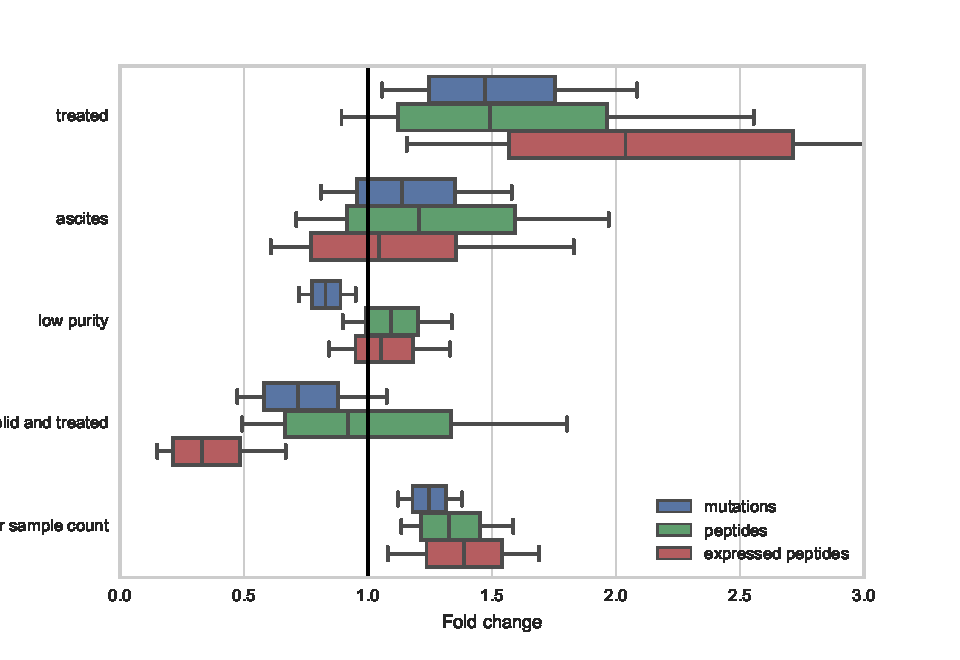
\includegraphics[scale=1.0]{figures/bayesian_model_effects.pdf}
\caption{Bayesian model effects. }
\label{fig:bayesian}
\end{figure}

\begin{figure}
\centering
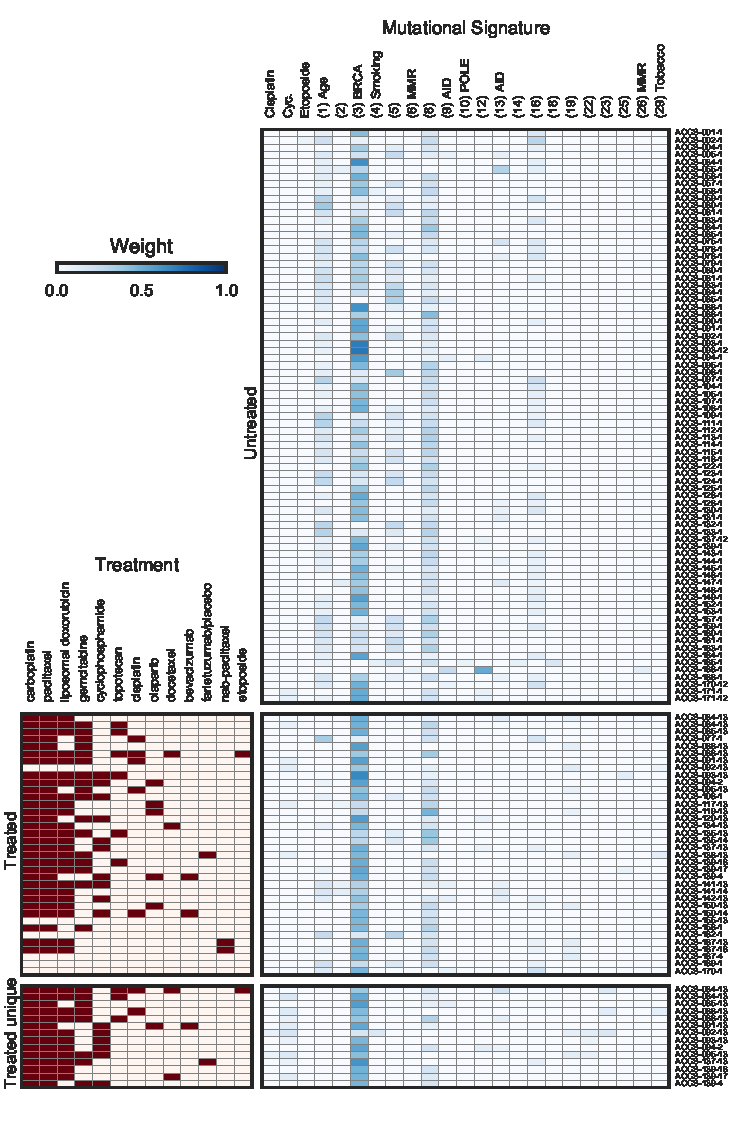
\includegraphics[scale=1.0]{figures/signatures.pdf}
\caption{Mutational signature deconvolution. }
\label{fig:signature}
\end{figure}




\section*{Discussion}

The fraction of cancer cells harboring a neoantigen may be critical in its ability to be targeted by a T cell response \cite{McGranahan_2016}.

\section*{Limitations}
RNA with hard thresholds to detect expressed peptides is subject to confounding by changes in gene expression -- e.g. if something gets upregulated post treatment





